\cotefile{138}
\scanpage{60}
\deleted{$C=(C_0,C_1)$ \unsure{groupoide|groupoïde} connexe

$G=\operatorname{Aut}(C)$ groupe des automorphismes

$G^0$ ss-groupe des $g\in G$ induisant l'identité sur $C_0$

\diagram{\begin{tikzcd}[ampersand replacement=\&,column sep=small]
1\arrow[r] \& G^0\arrow[r] \& G\arrow[r,swap,"\text{\uuline{surj}}"] \& \unsure{\mathfrak S|\mathscr S}_{C_0}\arrow[r] \& 1
\end{tikzcd}}

[ Pour qu'une \unsure{autoéquivalence} \inserted{$u$} soit un iso, il f et s. qu'elle soit bijective sur les objets de $C$, et induise un iso. \deleted{sur les} $\operatorname{Aut}(a)\longrightarrow\operatorname{Aut}(u(x))$ pour \uline{un} $x\in C_0$ ; d'autre part, pour toute application $C_0\overset{u_0}{\longrightarrow}C'_0$}

\diagram{\begin{tikzcd}[ampersand replacement=\&,column sep=small]
1\arrow[r,dash] \& \operatorname{Aut}^0(C)\arrow[r,dash] \& \operatorname{Aut} C\arrow[r,dash] \& \mathfrak S_C\arrow[r,dash] \& 1
\end{tikzcd}}

\[
\deleted{\operatorname{Aut}^0(C)\simeq}
\]
\diagram{\begin{tikzcd}[ampersand replacement=\&,column sep=small]
\unsure{0|o}\mathord{-}\cdot \\
1\arrow[r] \& \operatorname{Aut}^{\unsure{0}}(C,a)\arrow[r,dash] \& \operatorname{Aut}^0(C)\arrow[r,swap,"\unsure{1}"] \& \operatorname{Aut}\bigl(\underset{\substack{\Vert\\\operatorname{Aut}_C(a)}}{\pi_a}\bigr)\arrow[r] \& 1
\end{tikzcd}}

\deleted{A} Pour déterminer $\deleted{\operatorname{Aut}^0(C,a)=}$
\[
\operatorname{Aut}^0(C,a)=\bigl\{f\in\operatorname{Aut}(C)\mid \operatorname{Ob} f=\mathrm{id}\ :\bigl(f_a:\operatorname{Aut}(a)\longrightarrow\operatorname{Aut}(\underset{\substack{\Vert\\f(a)}}{a})\bigr)=\mathrm{id}\bigr\}
\]
On considère, pour tt $x\in C_0$,
\[
T_x=\operatorname{Isom}(a,x)\ ,\ \pi_a\text{-torseur à droite}
\]
et son commutant $\deleted{\unsure{G_x}}\operatorname{Aut}(x)$
% archive sheet number: 59
\scanpage{61}
\uline{Corollaire} Pour que $f$ soit un iso, il f. et s. que

a) $f$ induise
\[
\pi_0(f):\ \pi_0(C)\overset{\sim}{\longrightarrow}\pi_0(C')
\]

b) $f$ induise
\[
\unsure{\operatorname{Ob}|\operatorname{O}}f=f_0:\quad\operatorname{Ob}(C)\overset{\sim}{\longrightarrow}\operatorname{Ob}(C')
\]

c) $\forall i\in I\ ;\quad f_{a_i,a_i}:\operatorname{Aut}(a_i)\overset{\sim}{\longrightarrow}\operatorname{Aut}(f_0(a_i))$

\uline{NB} $f$ \unsure{équivalence|équivalen.} $\Longleftrightarrow$ a) et c) sont vrais

\uline{Corollaire} Pour qu'une application $f_0:C_0\longrightarrow C'_0$ provienne d'un iso $f:C\simeq C'$, il f. et s. que

a) $f_0$ \deleted{soit} bijective

b) $f_0$ transforme la relation d'équivalence de $C_0$ (\unsure{pour|par} comp. \unsure{connexes}) en celle de $C'_0$ (condition vide si $C,C'$ connexes)

c) $\forall i\in I$, $\operatorname{Aut}(f_0(a_i))$ est isom à $\operatorname{Aut}(a_i)$.

\begin{center}\rule{2em}{0.3pt}\end{center}

\deleted{\unsure{Se|So}} Supposons $C=C'$. Alors on trouve
\[
\operatorname{Aut}(C)\longrightarrow\unsure{\mathfrak S|\mathscr S}_{C_0}\qquad\text{\uline{surjective}}
\]
si $\operatorname{Aut}^0(C)$ est le noyau, on trouve donc
% archive sheet number: 60
\scanpage{62}
On trouve
\[
\operatorname{Aut}^0(C,a)\simeq\prod_{x\in C_0\setminus\{a\}}\deleted{\unsure{G_x}}\pi_x
\]

\figure{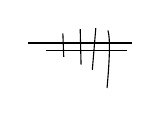
\begin{tikzpicture}[x=0.22cm,y=0.22cm]
\draw (-3,0)--(3,0) (-2,-.45)--(2.7,-.45);
\draw (-1,.55)--(-.95,-.8) (0,.8)--(.05,-1.25) (.9,.85)--(.7,-1.56) (1.6,.72) .. controls (1.8,.1) and (1.6,-2) .. (1.55,-2.6);
\end{tikzpicture}}

\deleted{Soit $K$ \unsure{un|le|des} graphe\unsure{,|.}}

Soit $I$ un ensemble muni d'une structure polygonale d'ordre $n\geq2$ \deleted{\unsure{i.e.} \unsure{$A_o$}} [pour $n=2$, il faut se donner l'un des \unsure{orbites|orientés} \inserted{de cardinal 2} $\deleted{\unsure{\Delta}}I^*$, \deleted{de cardinal 2, et} ou ce qui revient au $=$, $\Omega(\Pi)\simeq I\mathbin{\wedge}I^*\ \ldots$ ], $\mathbb D\ (\simeq\mathbb D_n)$ le groupe des autom. de $I$.

Soit $K=K(I)$ le graphe donné par
\[
\begin{aligned}
&\text{\uline{sommets} :}& \deleted{\unsure{O}}\Omega(\Pi)&=C_0=\{o,o'\}\\
&\text{\uline{arêtes}}& I&:\quad\text{(indexation $(\unsure{\ell|b}_i)_{i\in I}$)}
\end{aligned}
\]
\deleted{\unsure{Relation} d'incidence}

Incidence : \quad $C_0\times I$ (\unsure{tte|tt} arête incidente à \deleted{\unsure{tt o}}\inserted{tt sommet})

\inserted{$G$ opère sur $K(I)$, et on a aussi \deleted{\unsure{autre}} \inserted{l'involution} $\tau$ qui est l'identité sur $I$, et échange $o,o'$, commutant à $G$.}

\diagram{\begin{tikzcd}[ampersand replacement=\&,row sep=huge]
o\arrow[d,bend left=62,dash,"\ell_1"]\arrow[d,bend right=34,dash,double,swap,"\ell_0"]\arrow[d,bend right=61,dash,swap,"\ell_2"]\\
o'
\end{tikzcd}}

Soit $C(I)$ le groupoïde fondamental \unsure{du|de} $K(I)$. \deleted{le \unsure{gpe}} $G$ y opère par automorphismes, en opérant transitivement sur $C_0=\{o,o'\}$.

On va regarder le \deleted{commutant}\inserted{normalisateur de $G$} dans
% archive sheet number: 61
\scanpage{63}
$G$ dans $\operatorname{Aut}(C(I))$. On a un élément canonique $\tau$
% archive sheet number: 62
\scanpage{64}
\diagram{\begin{tikzcd}[ampersand replacement=\&,row sep=2.8ex,column sep=1.4em,arrows={line width=.48pt},execute at end picture={\draw[gray!40,very thin] (\tikzcdmatrixname-4-1.center) -- ($(\tikzcdmatrixname-4-1.center)+(-.85,0)$) -- ($(\tikzcdmatrixname-1-3.center)+(.92,-.16)$);}]
\& \& E^+
 \arrow[dddll,swap,"p_{20}^+",pos=.43]
 \arrow[dddrr,"p_{01}^+",pos=.45]
 \arrow[d,dashed,swap,"p_{12}^+",pos=.60]
 \arrow[ddl,dashed,swap,"\pi_2^+",near end]
 \arrow[ddr,dashed,"\pi_1^+",near end]
 \arrow[ddd,"\pi_0^+",near end]
 \arrow[dddrr,phantom,"\deleted{\unsure{\pi_1^+|p_{01}^+}}" description,very near end] \& \& \\
\& \& \unsure{D_{12}|\mathbb D_{12}}\arrow[dl,"q_{21}"]\arrow[dr,dashed,"q_{12}"] \& \& \\
\& S_2 \& \& S_1 \& \\
D_{20}\arrow[ur,"q_{20}"']\arrow[rr,"q_{02}"'] \& \& S_0 \& \& D_{01}\arrow[ul,dashed,"q_{10}"']\arrow[ll,"q_{01}"]\\
\& \& {} \& \& \\
\& \& {} \& \& \\
\& \& E^-\arrow[uuull,"p_{20}^-"]\arrow[uuurr,swap,"p_{01}^-"]
 \arrow[uuuuu,dashed,swap,"p_{12}^-",near start]\arrow[uuu,swap,"\pi_0^-"]
 \arrow[uuuul,dashed,"\pi_2^-",near end]\arrow[uuuur,dashed,swap,"\pi_1^-",near end] \& \&
\end{tikzcd}}

\[
\left\{\begin{aligned}
\rho_0^+&=(p_{01}^+)^{-1}p_{01}^-(p_{20}^-)^{-1}p_{20}^+\\
\rho_{\unsure{1|0}}^+&=(p_{12}^+)^{-1}p_{12}^-(p_{01}^-)^{-1}p_{01}^+\\
\rho_2^+&=(p_{20}^+)^{-1}p_{20}^-(p_{12}^-)^{-1}p_{12}^+
\end{aligned}\right.
\qquad \rho_2^+\rho_1^+\rho_0^+=\mathrm{id}_{E^+}
\]
\[
\begin{aligned}
S_0&\simeq E^+/\rho_0^+\simeq E^-/\rho_0^-\\
S_1&\simeq E^+/\rho_1^+\simeq E^-/\rho_{\unsure{1|0}}^-\\
S_2&\simeq E^{+}/\rho_{2}^+\simeq E^-/\rho_2^-
\end{aligned}
\]
\[
\left\{\begin{aligned}
\rho_{\unsure{2|0}}^-&=(p_{01}^-)^{-1}p_{01}^+(p_{20}^+)^{-1}p_{20}^-\\
\rho_1^-&=(p_{12}^{\deleted{\unsure{+}}-})^{-1}p_{12}^+(p_{01}^+)^{-1}p_{01}^-\\
\rho_2^-&=(p_{20}^-)^{-1}p_{20}^+(p_{12}^+)^{-1}p_{12}^-
\end{aligned}\right.
\]
% archive sheet number: 63
\scanpage{65}
Sous groupes finis de $G\unsure{\mathbb P|P}(1)$ (cas \uline{tame})

\margin{S.}
% archive sheet number: 64
\scanpage{66}
\inserted{cas galoisien $d_{ij}=\deleted{\unsure{N}}d_i=N/\unsure{\nu|v}_i$}
\[
\begin{aligned}
2-2g'&=N(2-2g)\deleted{\unsure{+}}-\underbrace{(N\nu\deleted{\unsure{+}}-\nu')}_{\sum_{i,j}(d_{ij}-1)}=N(2-2g)-\sum_i\underbrace{\nu_i(N/\nu_i-1)}_{N-\nu_i=N(1-\frac{\nu_i}{N})}
\end{aligned}
\]
$\deleted{\unsure{-\nu'}}$\qquad $\deleted{\unsure{-\nu}}$
\[
\boxed{2-2g'=N\left[(2-2g)-\sum_i\left(1-\frac1{d_i}\right)\right]}
\]
Si $g'=0$, on trouve $g=0$ et
\[
\boxed{\frac2N=2-\sum_i\left(1-\frac1{d_i}\right)>0}
\]
d'où
\[
\sum_i\left(1-\frac1{d_i}\right)<2
\]
\uline{OPS} Tous les $d_i\geq2$ \deleted{\unsure{car}} i.e. $I$ \uline{contient} \unsure{l'aire|l'ens.} de ramification

1) $\operatorname{Card} I=0$\qquad $\frac2N=2$, $N=1$ : \deleted{\unsure{grpe|pour}} $G=1$

2) $\operatorname{Card} I=1$
\[
\begin{aligned}
\frac2N&=2-\left(1-\frac1d\right)=1+\frac1d
&2&=N+\frac Nd=N+\nu\qquad\text{or }N\geq1,\ \nu\geq1\\
&&&&\text{donc }N=1,\nu=1\\
&&&& I=\varnothing
\end{aligned}
\]
\uline{impossible}

3) $\operatorname{Card} I=2$
\[
\begin{aligned}
\frac2N&=\frac1{d_1}+\frac1{d_2}& 2&=\frac N{d_1}+\frac N{d_2}=\nu_1+\nu_2
&\nu_1,\nu_2&\geq1\quad \nu_1=\nu_2=1\\
d_1&=d_2=N&&\text{\uline{$N$ quelconque}}
\end{aligned}
\]

4) $\operatorname{Card} I=3$\qquad $\deleted{\unsure{\frac2N=2}}$
\[
\frac1{\deleted{d_1}p}+\frac1{\deleted{d_2}q}+\frac1{d_3}>1\qquad
\left(\frac2N=\left(\frac1p+\frac1q+\frac1r-1\right)\right)
\]
OPS $\deleted{d_1}p\geq\deleted{d_2}q\geq\deleted{d_3}r$

a) $\deleted{\unsure{p}}r=2$\qquad $\frac1p+\frac1q>\frac12$\qquad i.e. \unsure{posant|posons} $p=\alpha+2,\ q=\beta+2$\qquad $(\alpha\geq\beta\geq0$\quad $\deleted{\unsure{\alpha}}$
\[
\begin{aligned}
2p+2q-pq&>0& \deleted{\unsure{2(\alpha+\beta)+8-}}&\\
&&\underbrace{2(\alpha+2)+2(\beta+2)-(\alpha+2)(\beta+2)}_{4-\alpha\beta>0}&>0\\
\alpha\beta&<4 &\deleted{\unsure{q}}\beta&=0,\ \deleted{\unsure{p}}\alpha\ \text{quelc.}\\
&&\deleted{\unsure{q}}\beta&=1,\ \deleted{\unsure{p}}\alpha=1,2,3\\
&&\deleted{\unsure{\beta=2,\ \alpha}}&
\end{aligned}
\]
\[
\left\{\begin{aligned}
&(2,2,p)& p\geq2&\quad\text{quelc.}& N&=2p\\
&(2,3,3)&&&N&=12\\
&(2,3,4)&&&N&=24\\
&(2,3,5)&&&N&=60
\end{aligned}\right.
\]

b) $r\geq3$\qquad $\frac1p+\frac1q>1-\frac1r\geq\frac23$\qquad \uline{impossible} car $\frac1p,\frac1q\leq\frac13$

5) $\operatorname{Card} I\geq4$\qquad $\deleted{\unsure{2-}}\ \frac1p+\frac1q+\frac1r+\frac1s>2$\qquad $\deleted{\unsure{\geq}}p\geq q\geq r\deleted{\unsure{\geq}}\geq s$

Faisons d'abord $\unsure{\operatorname{Card}|\operatorname{card}} I=4$
\[
\deleted{\frac1p+\frac1q+\frac1r>2-\frac1s=1+\left(1-\frac1s\right)\geq1+\left(1-\frac1p\right)>1}
\]
% archive sheet number: 65
\scanpage{67}
% letterhead
\noindent U N I V E R S I T E\hfill Montpellier, le 28 Juin 1978\\
DES SCIENCES ET TECHNIQUES\\
DU LANGUEDOC\\
\texttt{-{}-{}-{}-{}-{}-{}-{}-{}-{}-{}-{}-}\\
Service de la Scolarité\\
MR / GJ\\
Diffusion\quad : Liste A\\
N° : 4066

% printed form
\uline{AVIS DE SOUTENANCE D'UNE THESE DE DOCTORAT DE 3ème CYCLE}

\uline{( CHIMIE ORGANIQUE PHYSIQUE )}

\uline{Nom et prénom du candidat} :\qquad AURELLY Michèle

\uline{Titre de la thèse} : Application de la corrélation de Hammett à l'étude de l'énolisation des cétones en milieux basique et superbasique.

\uline{Date, heure et lieu de soutenance prévus} :\\
JEUDI 13 JUILLET 1978 à 16 Heures\\
Salle de cours n° 9 - U. S. T. L.

\uline{Nom du Directeur de thèse} :\\
Monsieur le Professeur LAMATY.

\uline{Désignation du laboratoire où la thèse est préparée} :\\
Laboratoire de Chimie Organique Physique.

\uline{Analyse de l'ouvrage} :

Ce travail consiste à cerner de plus près les mécanismes de l'énolisation des cétones par l'étude d'acétophénones et de méthyl-2 phényl-1 butanones-1 substituées, dans des milieux basiques. Les constantes p de Hammett ont été mesurées en fonction de la nature du milieu.

\uline{Durée approximative des recherches ayant abouti à la thèse : 3 ans.}

\uline{Composition du jury proposé} :\\
MM. :\\
LAMATY, Président\\
SCHUE\\
WYLDE\\
MION

Le Secrétaire Général,\\
\handwritten{\unsure{E Siau}}\\
\uline{E. SIAU}
% archive sheet number: 66
\scanpage{68}
\deleted{$(p,q,r)$ doit être parmi les \deleted{\unsure{trois}} syst. énumérés

a) $p,2,2$ : $\frac1p+\frac12+\frac12>\bigl(1+(1-\frac1s)\bigr)$ i.e. $\frac1p+\frac1s>1$ impossible car $\frac1p,\frac1s\leq\frac12$

b) $(p,3,2)$ $(p=3,4,5)$, $s\geq p$ $\deleted{\unsure{\frac1p+\frac13+\frac12|\frac1p+\frac1s+\frac12}}$
\[
\frac1s+\frac1p+\underbrace{\frac13+\frac12}_{5/6}>2\qquad \frac1s+\frac1p>\frac76\quad\text{impossible car }\frac1s,\frac1p\leq\frac13
\]}

\[
\frac1p+\frac1q>2-\underbrace{\left(\frac1r+\frac1s\right)}_{\substack{\leq1\\\text{car }\frac1r\leq\frac12\\\frac1s\leq\frac12}}\geq1
\quad\text{donc }\frac1p+\frac1q\geq1\quad\text{impossible car }\frac1p,\frac1q\leq\frac12
\]
\uline{Impossible} !

Car si $\operatorname{Card} I\geq4$, on \unsure{aura|aurait}
\[
\frac1{d_1}+\frac1{d_2}+\frac1{d_3}+\frac1{d_4}\deleted{\unsure{+\sum_{5\leq i\leq\nu}\frac1{d_i}}}>2\deleted{\unsure{-2}}+\sum_{5\leq i\leq\unsure{\nu|v}}\left(1-\frac1{d_i}\right)
\]
et on vient de voir que c'est impossible !\margin{$\unsure{\nu'|v'|v\text{.}}$\par $2$}

\deleted{\uline{Étude du cas} \deleted{$\operatorname{Card} I=2$}\inserted{$(N,N)$} : En caractéristique $0$, c'est le cas \unsure{kummerien}
\[
G\simeq\mu_N(k)\simeq\mathbb Z/N\mathbb Z\qquad\ldots
\]
\deleted{\unsure{Plus généralement}} \unsure{sim|sin}, il en est ainsi en car. $p$ première à $N$.

Si $p\mid N$, on trouve une \inserted{$p$-}extension \inserted{(de degré $p^r$, \unsure{tott|tolt} ramifiée et \unsure{isomorphe|séparable})} d'une $N'$-extension \unsure{kummerienne} $(N=p^rN',\ (p,N')=1)$. C'est donc une \uline{extension} \deleted{est} \uline{résoluble}, \inserted{mais mieux :} \deleted{\unsure{On en peut dire plus, sans étude approfondie. On obtient même la précision abélienne unitaire}} \deleted{Or} les $p$-\deleted{extensions} sous-groupes \inserted{$H$} de $\unsure{GP|G\mathbb P}(1,k)$ sont \uline{abéliens} et contenus dans \unsure{sous-groupe unipotent|sous-groupes unipotents} de dim $1$, \inserted{conjugués entre eux, et $H$ isom. à $(\mathbb Z/p\mathbb Z)^{\unsure{\nu|r}}$.} On trouve donc $G\subset\mathrm{Borel}$, et par suite $G$ produit $1/2$ direct d'un groupe cyclique premier à \unsure{2|?|p} car., par un $(\mathbb Z/p\mathbb Z)^r$. En fait, on voit aisément (\deleted{\unsure{si car $=$}} qu'on est soit dans le premier cas (cyclique premier à car, donc kummerien, qui n'est exclu), ou dans la \unsure{direction|deuxième}}

% slanted
\margin{\unsure{En tous les cas, on a une extension abélienne, soit kummerienne|En tous les cas, on a une extension abélienne, non kummerienne|En tous les cas, on a une extension résoluble, soit kummerienne} (d'allure \unsure{purement insép.|premier à $p$}), sauf \unsure{en type|que grpe} $(\mathbb Z/p^{\unsure{n|r}}\mathbb Z)^\nu$}

\deleted{\uline{Etude du cas} $(\deleted{\unsure{d}}N,2,2)$, $\{\,[G]=2N\,\}$. En car. $\ne2$, l'\uline{indice} \inserted{de} ramification $2$ \deleted{\unsure{de type modéré}} a ramification modérée, et faisant une extension kummerienne de degré $2$, on \deleted{\unsure{trou}} trouve un $X'/Y'$ qui n'a plus que $2$ pts de ramification \deleted{\unsure{dans}} $Y'$, donc $X'/Y'$ est justiciable de l'étude précédente mais \deleted{\unsure{il}} faut vérifier \deleted{\unsure{si tel est si}} \unsure{que} $X'$ de genre $0$ (facile)}

\diagram{\begin{tikzcd}[ampersand replacement=\&,column sep=small,row sep=small]
X \& X'\arrow[l,dash]\arrow[d,dash]\\
Y \& Y'\arrow[l,dash]
\arrow[from=1-1,to=2-1,dash]
\end{tikzcd}}
% archive sheet number: 67
\scanpage{69}
% letterhead
\noindent U N I V E R S I T E\hfill Montpellier, le 26 Juin 1978\\
DES SCIENCES ET TECHNIQUES\\
DU LANGUEDOC\\
\texttt{-{}-{}-{}-{}-{}-{}-{}-{}-{}-{}-{}-}\\
Service de la Scolarité\\
MR/GJ\\
Diffusion : Liste A\\
N°:4000

% printed form
\uline{AVIS DE SOUTENANCE D'UNE THESE DE DOCTORAT D'UNIVERSITE}

\uline{Nom et prénom du candidat} : PAYEN Jean-Luc

\uline{Titre de la thèse} : Contribution à l'étude de la protection des surfaces métalliques par les composés oxyfluorés du phosphore V.

\uline{Date, heure et lieu de soutenance prévus} :\\
13 JUILLET 1978 à 11 Heures\\
Ecole Nationale Supérieure de Chimie.

\uline{Nom du Directeur de thèse} :\\
Monsieur le Professeur L. COT.

\uline{Désignation du laboratoire où la thèse est préparée} :\\
Laboratoire de Chimie minérale appliquée - Chimie des Matériaux, \quad E. N. S. C. M.

\uline{Analyse de l'ouvrage} :

Les sels de l'anion $\mathrm{PO3F}^{2-}$ peuvent être utilisés lors de l'opération de post-traitement après phosphatation en substitution des sels de chrome VI hautement toxiques.

Une étude de la nature de la surface crée par phosphatation et passivation par $\mathrm{K2PO3F}$ a été entreprise par différentes techniques : ESCA,Microscopies électronique , et ionique. Elle montre une réorganisation physico chimique de la couche.

\uline{Durée approximative des recherches ayant abouti à la thèse} : 2 ans

\uline{Composition du jury proposé} :\\
MM.\qquad :\\
M.\quad MAURIN\\
L.\quad COT\\
P.\quad DESRE\\
J.\quad DURAND\\
X.\quad GRANDIN DE L'EPREVIER\\
B.\quad PARANT\\
P.R\quad PHILIP

Le Secrétaire Général,\\
\handwritten{\unsure{E Siau}}\\
\uline{E. SIAU}
% archive sheet number: 68
\scanpage{70}
Paradigme \deleted{\unsure{topologiques|topologique}}\inserted{``gruppentheoretisch''} des surfaces compactes à opérateurs.
% archive sheet number: 69
\scanpage{71}
Paradigme des courbes algébriques

I\quad Point de vue topologique.

On considère des surfaces topologiques (sans bord) orientables paracompactes \inserted{$X$} -- on se donne aussi un ensemble \inserted{$\omega$} de cardinal $2$, et on pose
\[
T=\mathbb Z\mathbin{\wedge}_{\mathbb Z/2}\omega\ ,
\]
et on suppose donnée pour $X$ une $\omega$-orientation, i.e. une \inserted{$\mathbb Z/2$-}application \deleted{\unsure{compatible}}\inserted{de $\omega$ dans} l'ens des orientations de $X$, ou ce qui revient au $=$, un isomorphisme du faisceau des entiers tordus sur $X$ avec le faisceau constant $T_X$. On suppose que \deleted{\unsure{les}}tte composante\deleted{s} connexe\deleted{s} $X_i$ de $X$ \deleted{sont}\inserted{est} homéomorphes à un $\hat X_i\setminus S_i$, où $\hat X_i$ est une surface compacte, et $S_i$ une partie finie de $\hat X_i$. On sait que $(\hat X_i,S_i)$ est déterminé à isom unique près par $X_i$ (comme le \unsure{décomp.|découpe|découpé} du compactifié de Čech
% archive sheet number: 70
\scanpage{72}
de $X_i$ suivant \unsure{son point|sa partie} à l'infini\ldots). Chaque $\hat X_i$ est automatiquement $\omega$-orienté, donc aussi
\[
\hat X=\coprod\hat X_i
\]

De cette façon, la catégorie envisagée (des surfaces topologiques ``spéciales'' $\omega$-orientées \inserted{-- avec \deleted{\unsure{leurs}}\unsure{homéomorphismes} $\omega$-orientés}) devient équivalente à celle des surfaces topologiques \inserted{$\omega$-orientées} à comp. conn. compactes \uline{munies} d'une partie \deleted{\unsure{f}} $S$ discrète, avec les isom. de couples $(\hat X,S)$.

De $\overline{\mathrm m}$, la catégorie des couples $\deleted{\unsure{(X,S)|(X,o,S)}}$ $(X,o,J)$ avec $(X,o)$ comme dessus ($o$ la $\omega$-orientation) et $J$ partie discrète de $X$, est équivalente à celle des systèmes $(\hat X,o,S,J)$, où $(\hat X,o)$ est une surface $\omega$-orientée à comp. conn compactes,
% archive sheet number: 71
\scanpage{73}
et $S,J$ sont deux parties discrètes disjointes de $\hat X$.

On va \deleted{\unsure{en}} passer aux catégories isotopiques correspondantes, et en donner des interprétations en termes de théorie des groupes. Bien entendu, pour cette description, on est ramené au cas connexe. On peut \deleted{aussi} noter tt de suite que pour ce pb, on est ramené au cas où $J=\varnothing$ [en \deleted{remplaçant}\inserted{\unsure{donnant|décrivant}} dans le cas général comme celui de la donnée d'un $(\hat X,I)$ \uline{plus} la donnée d'une partie $J$ de $I$]. Mais on gardera le pb sous \inserted{la} forme générale, en gardant également la dissymétrie dans le rôle des $S,J$ -- mais
% archive sheet number: 72
